\documentclass[11pt]{article}
\usepackage[cm]{fullpage}
\usepackage{amsmath,amssymb}
\usepackage{graphicx}
\usepackage{color}
\usepackage{algorithm}
\usepackage{algcompatible}
\usepackage[relative,overlay]{textpos}
\usepackage[colorlinks,bookmarksopen,bookmarksnumbered,citecolor=red,urlcolor=red,breaklinks=true]{hyperref}
\newcommand{\cblue}[1]{{\color{blue}#1}}
\renewcommand{\vec}[1]{{#1}}
\newcommand{\figdir}{./figures/}
\newcommand{\note}[1]{\cblue{NOTE: #1}}
\author{Eike Mueller, University of Bath}
\date{\today}
\title{Multilevel Monte Carlo for Quantum Field Theories on the Lattice}
\begin{document}
\maketitle
%%%%%%%%%%%%%%%%%%%%%%%%%%%%%%%%%%%%%%%%%%%%%%%%%%%%%%%%%%%%%%%%%%%%%%%%%
\section{Motivation and Overview}
%%%%%%%%%%%%%%%%%%%%%%%%%%%%%%%%%%%%%%%%%%%%%%%%%%%%%%%%%%%%%%%%%%%%%%%%%
By using Feynman's path integral formulation of quantum mechanics \cite{Feynman2010}, lattice field theories predict the fundamental properties and interactions of subatomic particles. Numerical results are obtained by Markov Chain Monte Carlo (MCMC) sampling of discretised fields on a space-time grid. To produce physically relevant results, both the number of lattice points and the number of Monte Carlo samples have to be increased, making accurate simulations challenging.

The Multilevel Monte Carlo (MLMC) algorithm \cite{Heinrich2001,Giles2008,Giles2015} has been shown to lead to a considerable reduction in computational cost in a wide range of applications (see e.g. \cite{Muller2015,Katsiolides2017}). The key idea is to construct coarse grained versions of the problem at hand which accelerate sampling without introducing any additional bias errors. It should be stressed that MLMC is a proper variance reduction technique and goes beyond other hierarchical approaches such as \cite{Faas1986} which create ``better'' samples but do not reduce the computational complexity.

Recently the multilevel approach has been adapted to an Markov Chain MC setting in \cite{Dodwell2015}. We aim to apply the same methods in the context of lattice field theory, exploiting the natural hierarchy of coarse grained effective theories obtained by renormalisation. In contrast to the Standard Monte Carlo (StMC) method, the computational complexity of MLMC is independent of the space-time dimension $d$. This makes the approach particularly promising for larger $d$, such as five-dimensional domain-wall fermion formulations \cite{Kaplan1992} of QCD. 
%%%%%%%%%%%%%%%%%%%%%%%%%%%%%%%%%%%%%%%%%%%%%%%%%%%%%%%%%%%%%%%%%%%%%%%%%
\section{Methods}
%%%%%%%%%%%%%%%%%%%%%%%%%%%%%%%%%%%%%%%%%%%%%%%%%%%%%%%%%%%%%%%%%%%%%%%%%

%%%%%%%%%%%%%%%%%%%%%%%%%%%%%%%%%%%%%%%%%%%%%%%%%%%%%%%%%%%%%%%%%%%%%%%%%
\subsection{Lattice Field Theory}
%%%%%%%%%%%%%%%%%%%%%%%%%%%%%%%%%%%%%%%%%%%%%%%%%%%%%%%%%%%%%%%%%%%%%%%%%
Let $\theta=\theta(x)$ be a scalar quantum field which is defined at any point $x$ in a $d$-dimensional unit box. The expectation value $\langle Q\rangle$ of a physical observable (or ``quantity of interest'') $Q=Q[\theta]$ can be written as a sum over all possible field configurations $\theta$ weighted by the exponential of the action $S[\theta]$ ($Z$ is a normalisation constant):
\begin{equation}
  \langle Q\rangle = Z^{-1} \int_{\text{all $\theta$}} Q[\theta]e^{-S[\theta]}\;d\theta \approx \frac{1}{N} \sum_{n=1}^N Q[\theta_L^n] = \hat{Q}^{\text{StMC}}_{L,N} \qquad\text{where}\quad \mathbb{R}^{M}\ni \theta_L^n\sim e^{-S[\cdot]}\label{eqn:StMCestimator}
\end{equation}
In this equation two approximations are made to obtain an estimator $\hat{Q}^{\text{StMC}}_{L,N}$ for $\langle Q\rangle$:
\begin{itemize}
\item \textbf{Discretisation}. The field $\theta$ is represented by its values $(\theta_L)_{j\in [1,\dots,M]}$ at the $M=2^{L\cdot d}$ points of a $d$-dimensional space-time lattice with spacing $a=2^{-L}$. The resulting bias error is $\mathcal{O}(a^\alpha)=\mathcal{O}(M^{-\alpha/d})$ where $\alpha$ is the order of the discretisation (typically $\alpha=1,2$).
    \item \textbf{Monte Carlo integration}. The integral is evaluated by summing the value of the observable for $N$ random fields $\{\theta_L^n\}_{n=1}^N$ which are distributed according to $e^{-S[\cdot ]}$. The sampling error is $\propto{1/\sqrt{N}}$.
\end{itemize}
Sophisticated methods such as Hybrid MC \cite{Duane1987} (to reduce autocorrelations in the Markov chain) and improved actions \cite{Lepage1994} (to increase the discretisation order $\alpha$) have been developed to minimise both errors.
The computational cost to calculate $\langle Q\rangle$ to accuracy $\epsilon$ by reducing both errors below $\frac{1}{2}\epsilon$ is $\text{C}^{\text{StMC}}\propto N\cdot M=\mathcal{O}(\epsilon^{-2-d/\alpha})$. As shown in \cite{Dodwell2015} Markov chain MLMC has the potential to reduce this cost to $\mathcal{O}(\epsilon^{-2}|\log(\epsilon)|)$.
%%%%%%%%%%%%%%%%%%%%%%%%%%%%%%%%%%%%%%%%%%%%%%%%%%%%%%%%%%%%%%%%%%%%%%%%%
\subsection{Multilevel Monte Carlo}
%%%%%%%%%%%%%%%%%%%%%%%%%%%%%%%%%%%%%%%%%%%%%%%%%%%%%%%%%%%%%%%%%%%%%%%%%
The key idea in Multilevel Monte Carlo is to construct a set of auxilliary models for fields $\theta_\ell$ and $\Theta_\ell$ on levels $\ell=L-1,\dots,0$ which are defined on coarser lattices (see Fig. \ref{fig:multilevel}, left).
\begin{figure}
  \begin{center}
  \begin{minipage}{0.55\linewidth}
    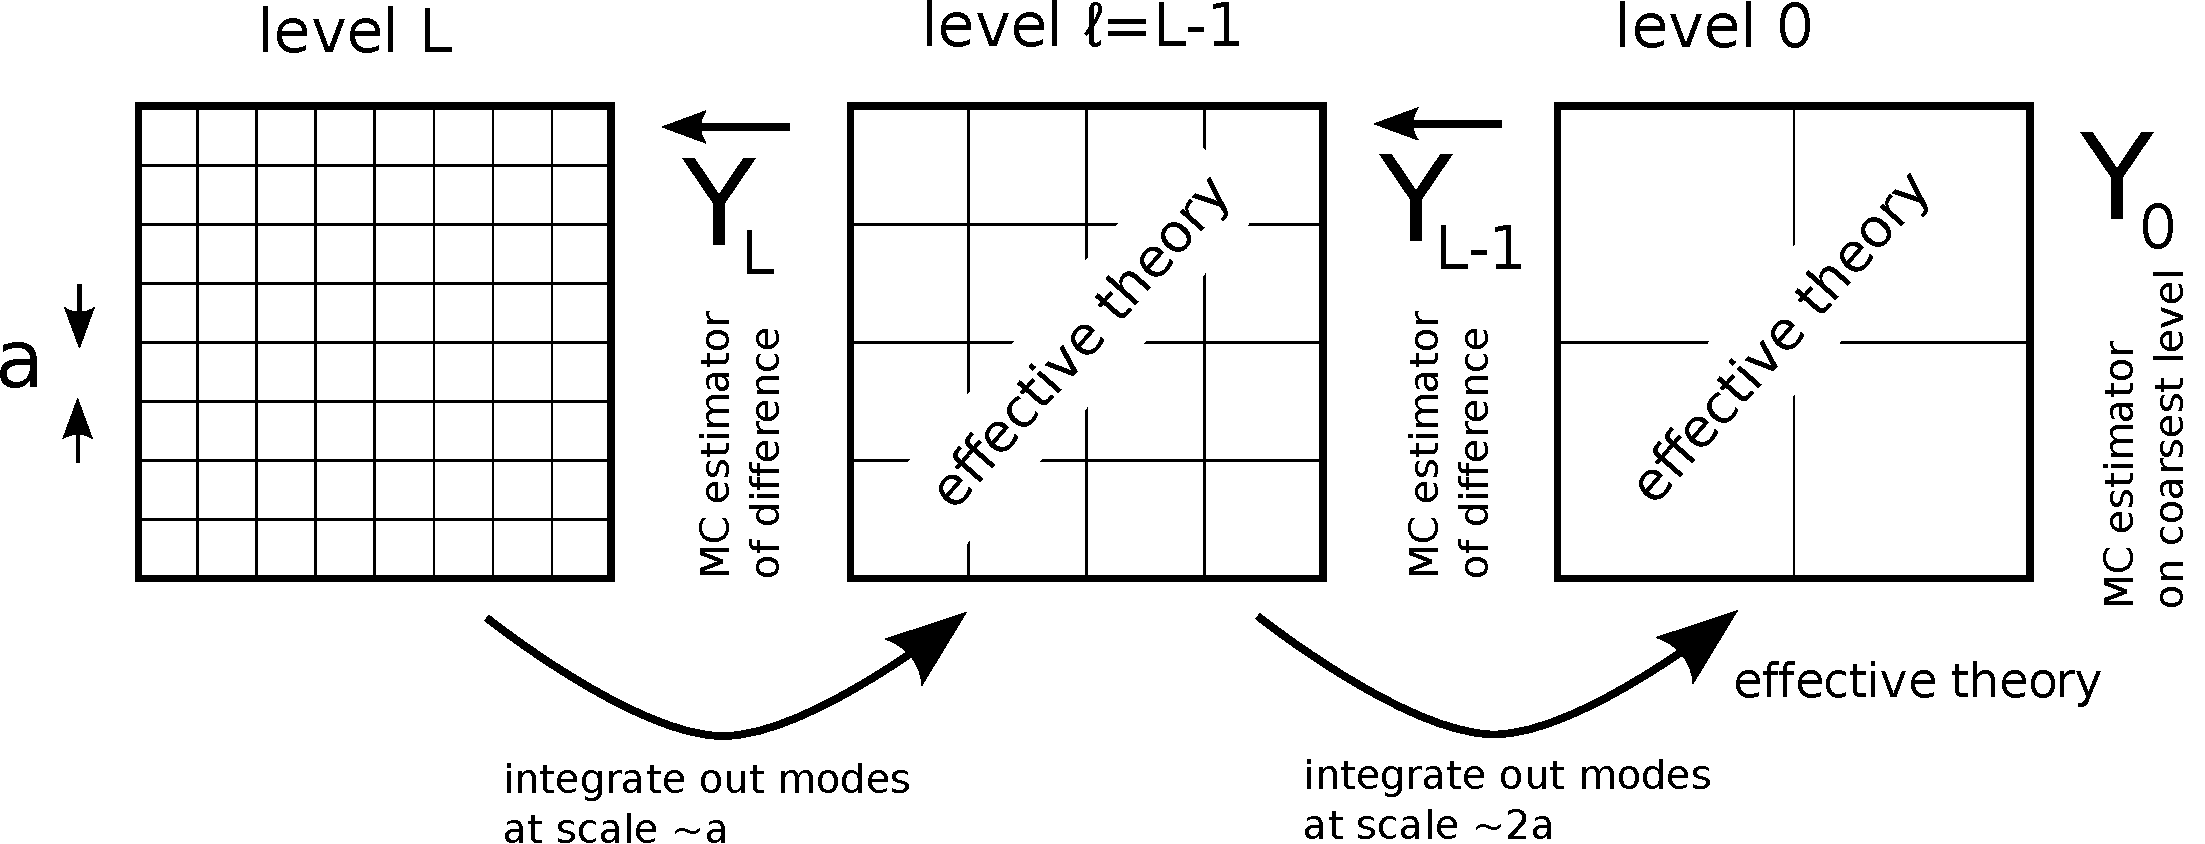
\includegraphics[width=\linewidth]{\figdir/multilevel_schematic.pdf}
  \end{minipage}
  \hfill
  \begin{minipage}{0.4\linewidth}
    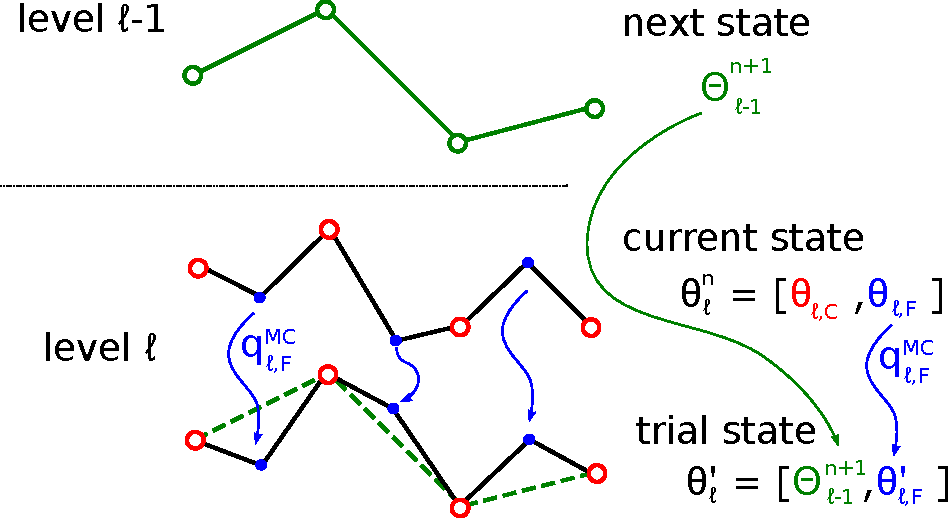
\includegraphics[width=\linewidth]{\figdir/multilevel_paths.pdf}
  \end{minipage}
  \caption{Multilevel hierarchy of grids for $L=2$ levels (left) and hierarchical sampling of paths (right).}\label{fig:multilevel}
  \end{center}
\end{figure}
By calculating differences in the observables between subsequent levels the following estimator can be written down as a telescoping sum of difference estimators $\hat{Y}^{\text{MC}}_{\ell,N_\ell}$
\begin{equation}
  \hat{Q}_{L,\{N_\ell\}}^{\text{MLMC}} := \hat{Q}_{0,N_0}^{\text{StMC}} + \sum_{\ell=1}^L \hat{Y}_{\ell,N_\ell}^{\text{MC}}\qquad\text{with}\quad
  \hat{Y}_{\ell,N_\ell}^{\text{MC}} :=  \frac{1}{N_\ell}\sum_{n=1}^{N_\ell} \left(Q_\ell[\theta_\ell^n] - Q_{\ell-1}[\Theta_{\ell-1}^n]\right).\label{eqn:MLMCestimator}
\end{equation}
It is important to note that by construction the bias of the multilevel estimator $\hat{Q}_{L,\{N_\ell\}}$ in Eq. (\ref{eqn:MLMCestimator}) is the same as the (fine level) estimator in Eq. (\ref{eqn:StMCestimator}) since the samples $\{\theta_\ell^n\}$ and $\{\Theta_\ell^n\}$ are drawn from the same distribution. By choosing the number of samples $N_\ell$ on each level appropriately, the cost is greatly reduced for two reasons:
\begin{enumerate}
\item \textbf{Variance decay.} Only the difference $Y_\ell$ of the observable on two subsequent levels is estimated. Since this difference has a much smaller variance than the observable itself, much fewer Monte Carlo samples are required. This is confirmed in Fig. \ref{fig:quantum_results} for a simple quantum system.
  \item \textbf{Reduced coarse level cost.} Since the number of lattice sites on coarse levels is much smaller, especially in high dimensions, sampling on those levels is significantly cheaper. In some cases the computational work is concentrated on the coarsest level where a large number of samples can be generated cheaply.
\end{enumerate}
As shown in the Complexity Theorem in \cite{Dodwell2015}, the computational cost of the multilevel version of MCMC sampling can be reduced to up to $C^{\text{MCMC}}=\mathcal{O}(\epsilon^{-2}|\log(\epsilon)|)$, provided the variance of the difference decays as $\text{Var}[Y_\ell]\propto M_\ell^{-\beta}$. This requires requires suitable coupling between the Markov chains $\theta_\ell^n$ and $\Theta_{\ell-1}^n$ on subsequent levels; an algorithm for this is described in \cite{Dodwell2015}. We have implemented this algorithm for a simple one-dimensional quantum system with quartic potential $V$ (compare \cite{Creutz1981}). In this case the action on level $\ell$ with lattice spacing $a_\ell=2^{L-\ell}a \gg a$ and $M_\ell=2^{\ell-L}M \ll M$ time slices is
\begin{equation}
  S\left[\theta_\ell\right] = \sum_{j=1}^{M_\ell} a_\ell\left\{\frac{m_0}{2}\left(\frac{(\theta_\ell)_j-(\theta_\ell)_{j-1}}{a_\ell}\right)^2 + V\left((\theta_\ell)_j\right)\right\}\qquad \text{with}\quad V(\theta) = \frac{1}{2}m_0\mu^2\theta^2+\frac{1}{4}\lambda\theta^4.\label{eqn:quantum_action}
\end{equation}
As Fig. \ref{fig:multilevel} (right) illustrates, in the Metropolis algorithm the fine level trial state $\theta'_\ell=[\theta'_{\ell,C},\theta'_{\ell,F}]$ is constructed by taking the values $\theta'_{\ell,C}$ at the even nodes from the next coarse level path $\Theta_\ell^{n+1}$. The odd modes $\theta'_{\ell,F}$ are drawn from an approximate quadratic action $q_{\ell}^{\text{MF}}$ conditioned on the coarse modes. A subsequent Metropolis accept/reject step with the fine level action ensures that the next state $\theta_\ell^n$ in the fine level Markov chain is drawn from the correct distribution; this guarantees the telescoping-sum property and avoids additional bias.

As Fig. \ref{fig:quantum_results} confirms, the variance of the differences $Y_\ell$ decays $\propto M_\ell^{-2}$ or $\propto M_\ell^{-1}$ and is much smaller than the variance of the observable itself both for the harmonic oscillator ($\mu^2=1$, $\lambda=0$) and for a double-well potential ($\mu^2=-1$, $\lambda=1$). In the latter case the coarse modes $\Theta_{\ell-1}$ are sampled using Hybrid Monte Carlo \cite{Duane1987}.
\begin{figure}
  \begin{center}
  \begin{minipage}{0.45\linewidth}
    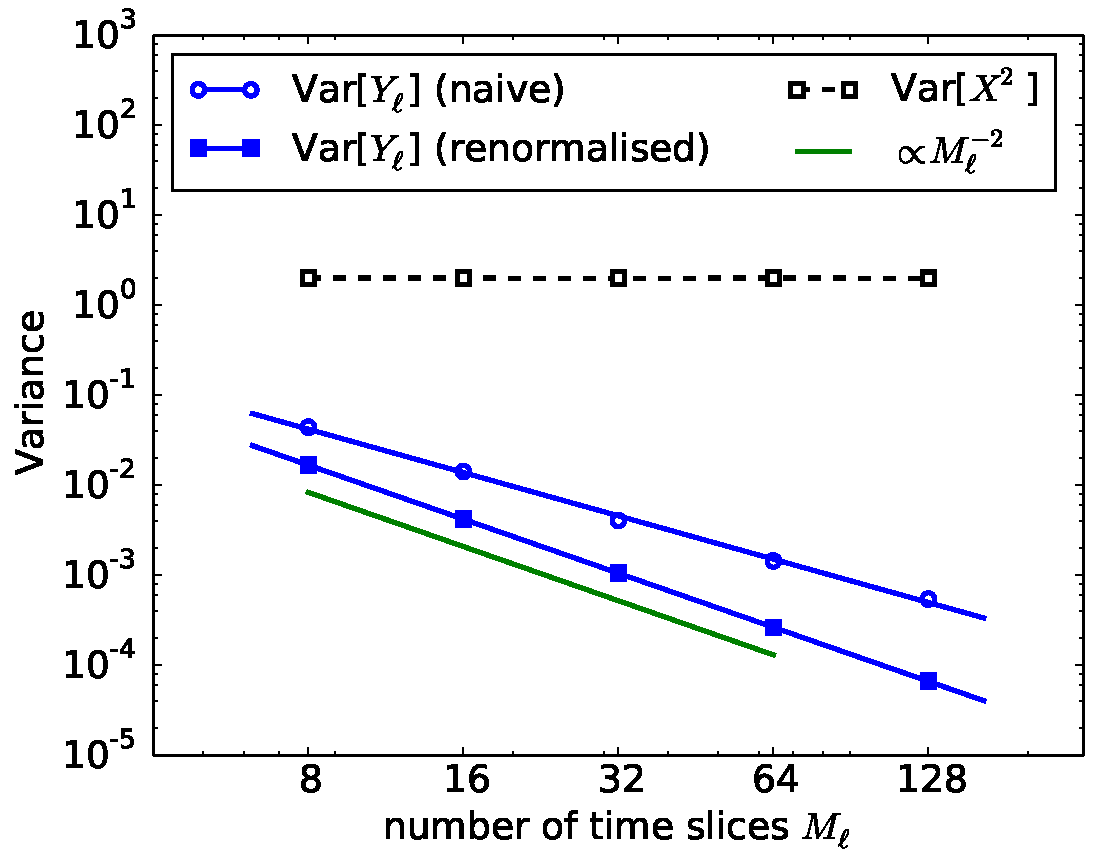
\includegraphics[width=\linewidth]{\figdir/variance_decay_ho.pdf}
    \begin{textblock}{4.0}(1.25,-1.0)
      $V(\theta)=\frac{1}{2}\theta^2$
    \end{textblock}
    \begin{textblock}{4.0}(4.25,-2.5)
      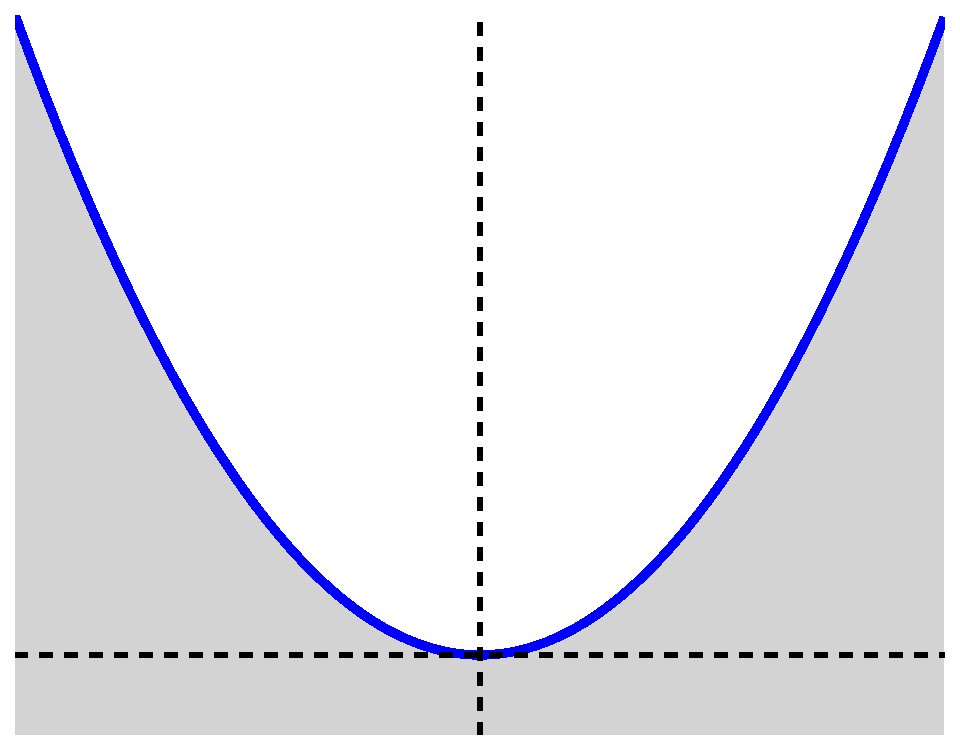
\includegraphics[width=0.4\linewidth]{\figdir/potential_harmonic.pdf}
    \end{textblock}
  \end{minipage}
  \hfill
  \begin{minipage}{0.45\linewidth}
    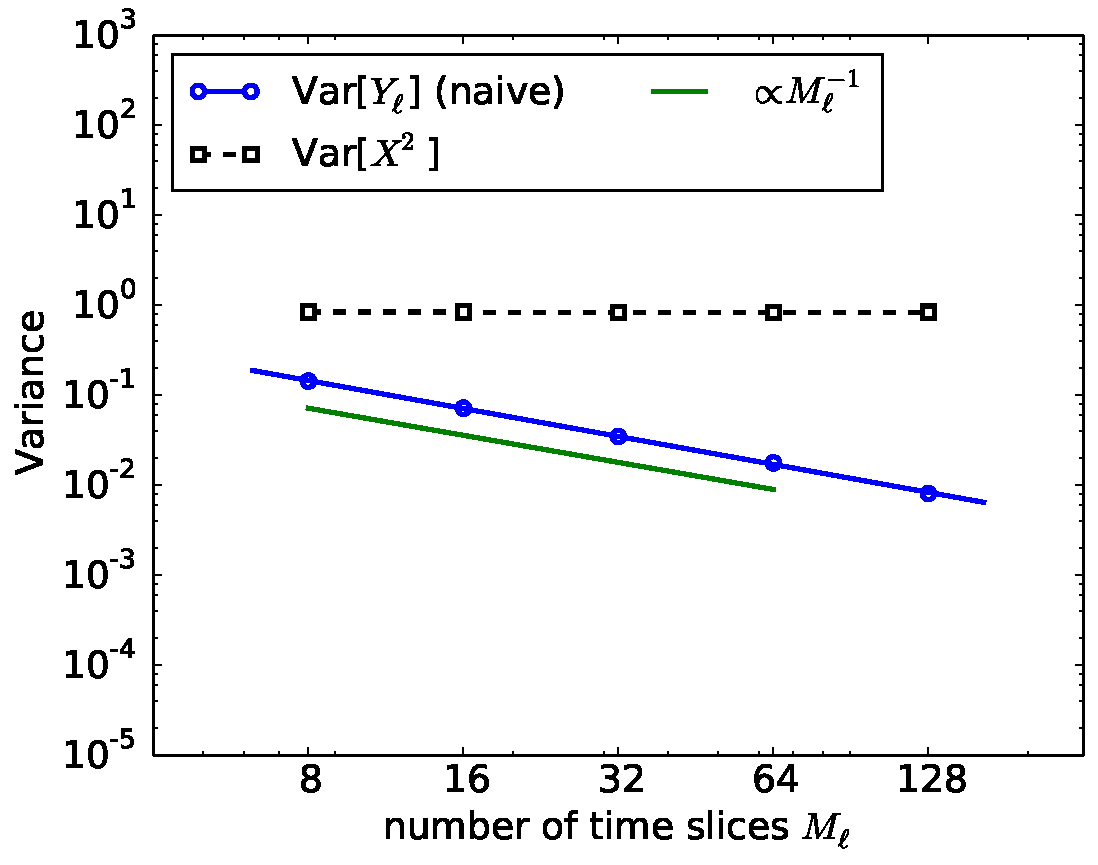
\includegraphics[width=\linewidth]{\figdir/variance_decay_qo.pdf}
    \begin{textblock}{4.0}(1.25,-1.0)
      $V(\theta)=-\frac{1}{2}\theta^2+\frac{1}{4}\theta^4$
    \end{textblock}
    \begin{textblock}{4.0}(4.25,-1.5)
      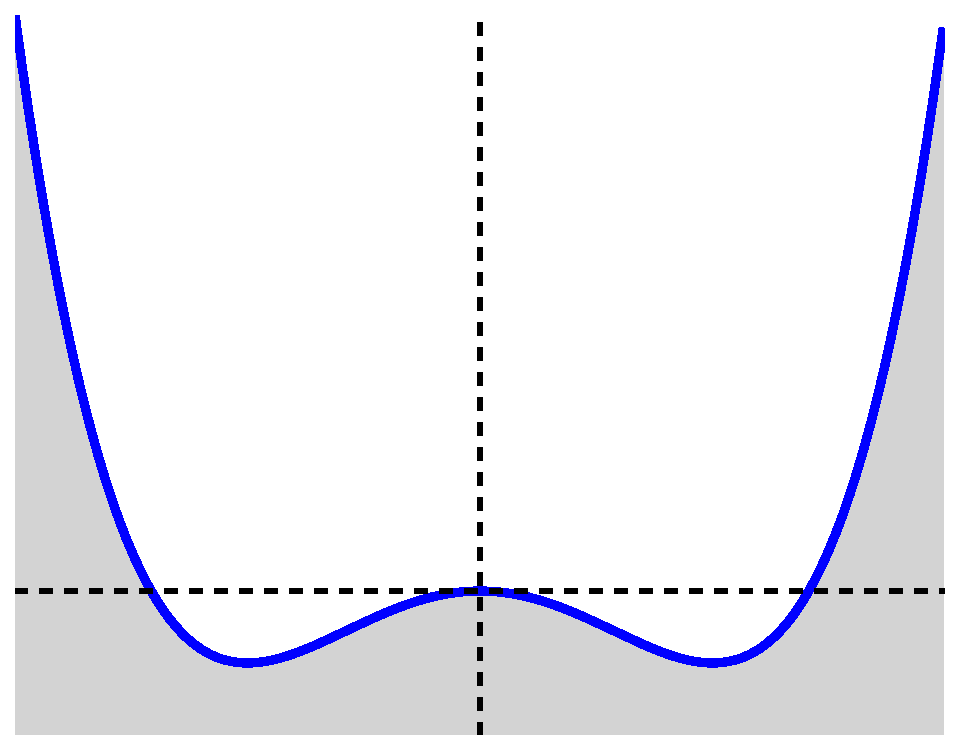
\includegraphics[width=0.4\linewidth]{\figdir/potential_quartic.pdf}
    \end{textblock}
  \end{minipage}
  \caption{Variance decay of difference estimator $Y_\ell$ between subsequent levels $\ell$ for the harmonic oscillator (left) and quartic double-well potential (right). The (much larger) variance of the observable $X^2$ itself is shown as a dashed line at the top.}
  \label{fig:quantum_results}
  \end{center}
\end{figure}
%%%%%%%%%%%%%%%%%%%%%%%%%%%%%%%%%%%%%%%%%%%%%%%%%%%%%%%%%%%%%%%%%%%%%%%%%
\subsection{Effective Field Theories and Renormalisation}
%%%%%%%%%%%%%%%%%%%%%%%%%%%%%%%%%%%%%%%%%%%%%%%%%%%%%%%%%%%%%%%%%%%%%%%%%
To guarantee optimal coupling between subsequent levels and hence reduce the variance $Y_\ell$ requires that the theories on the subsequent levels are ``similar''. In other words, the theory on level $\ell-1$ should describe the same physics as the slowly varying, low energy modes on level $\ell$. This is the concept of an effective theory: the coarse theory on level $\ell-1$ is obtained by integrating out the quantum fluctuations of high frequency modes on level $\ell$. For some cases (harmonic oscillator or free quantum field) this can be done exactly. As Fig. \ref{fig:quantum_results} (left) demonstrates, this leads to a further variance reduction and thus increased performance of the MLMC algorithm. Neglecting irrelevant operators, the parameters of the coarse level theory (e.g. $m_0$, $\mu$ and $\lambda$ in Eq. (\ref{eqn:quantum_action})) can be obtained by the renomalisation group transformation from scale $a_\ell$ to $a_{\ell-1}$. Due to the great practical relevance of Quantum Chromodynamics (QCD), asymptotically free theories are of particular interest. In this case there is a well developed machinery for lattice perturbation theory, see e.g. \cite{Hart2009}. Other cases of interest are theories close to a finite non-trivial critical point where the parameters are scale invariant, but naive Markov chain Monte Carlo sampling is very challenging due to long range correlations.
%%%%%%%%%%%%%%%%%%%%%%%%%%%%%%%%%%%%%%%%%%%%%%%%%%%%%%%%%%%%%%%%%%%%%%%%%
\section{Workplan}
%%%%%%%%%%%%%%%%%%%%%%%%%%%%%%%%%%%%%%%%%%%%%%%%%%%%%%%%%%%%%%%%%%%%%%%%%
Ultimately the goal will be to apply Multilevel Monte Carlo techniques to lattice QCD. Since this theory is non-trivial (the field is not a scalar and the action is invariant under local gauge transformation, i.e. the probability density is constant on submanifolds), we will apply the methods to models of increasing complexity:
\begin{enumerate}
\item Study one-dimensional quantum systems and extend the results in Fig. \ref{fig:quantum_results} to construct a multilevel MCMC sampler in those cases. While important to sketch out the general methods, MLMC is likely to achieve gains mainly for small $\epsilon$ since $d=1$ and we only expect at gain of $\epsilon^{-1/\alpha}/|\log(\epsilon)|$ (as the calculation in the appendix of \cite{Creutz1981} shows, $\alpha=2$ for the harmonic oscillator).
\item Extend this to higher-dimensional systems such as the (exactly renormalisable) free field in $d$-dimensions or the asymptotically free non-linear sigma model. Since the cost of the standard Monte Carlo method grows $\propto \epsilon^{-2-d/\alpha}$ this will give more relatistic estimates of achievable gains.
\item Investigate the application in lattice QCD. One particular challenge here is ensuring that coupling between subsequent levels does not break gauge invariance.
\end{enumerate}
\bibliographystyle{unsrt}
{\footnotesize
  \bibliography{plan}
}
\end{document}
